\documentclass[pdflatex,compress,mathserif]{beamer}

%\usetheme[dark,framenumber,totalframenumber]{ElektroITK}
\usetheme[darktitle,framenumber,totalframenumber]{ElektroITK}

\usepackage[utf8]{inputenc}
\usepackage[T1]{fontenc}
\usepackage{lmodern}
\usepackage[english]{babel}
\usepackage{amsmath}
\usepackage{amsfonts}
\usepackage{amssymb}
\usepackage{graphicx}
\usepackage{multicol}
\usepackage{lipsum}
\usepackage{framed}
\usepackage{minted}

\definecolor{LightGray}{gray}{0.95}

\usefonttheme[onlymath]{serif}

\newcommand*{\Scale}[2][4]{\scalebox{#1}{$#2$}}%

\setbeamertemplate{caption}[numbered]

\title{Digital Signal Processing}
\subtitle{Fast Fourier Transform (FFT)}

\author{Mifta Nur Farid}
\date{Sept. $\text{4}^\text{st}$, 2023}

\begin{document}

\maketitle

\section{Introduction}

\begin{frame}{Fast Fourier Transform (FFT)}
	\begin{itemize}
		\item very efficient algorithm in computing DFT coefficients $X(k)$
		\item can reduce a very large amount of computational complexity (multiplications)
		\item consider the digital sequence $x(n)$ consisting of $2^m$ samples, where $m$ is a positive integer
		\begin{itemize}
			\item $N = 2, 4, 8, 16, \text{ etc}$
			\item  If $x(n)$ does not contain $2^m$ samples, then we simply append it with zeros until the number of the appended sequence is a power of 2
		\end{itemize}
	\end{itemize}
\end{frame}

\begin{frame}{Fast Fourier Transform (FFT)}
	\begin{itemize}
		\item Consider $x(n) = [1, 2, 3]$. Can we do the FFT to $x(n)$? \pause \textbf{No} \pause
		\item Because $x(n)$ does not contain $2^m$ samples \pause
		\item Solution? \pause \textbf{Append it with zeros}, $x(n) = [1,2,3,0]$
	\end{itemize}
\end{frame}

\begin{frame}{Fast Fourier Transform (FFT)}
	\begin{itemize}
		\item we focus on two formats of the radix-2 FFT algorithms:
		\begin{enumerate}
			\item The decimation-in-frequency algorithm
			\item The decimation-in-time algorithm
		\end{enumerate}
	\end{itemize}
\end{frame}

\section{Decimation-in-frequency algorithm}

\begin{frame}{Decimation-in-frequency algorithm}
	\begin{itemize}
		\item DFT:
		\begin{center}
			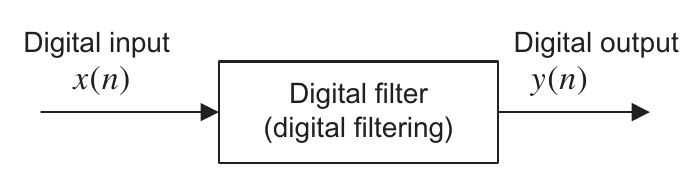
\includegraphics[width=0.7\linewidth]{img/img01}
			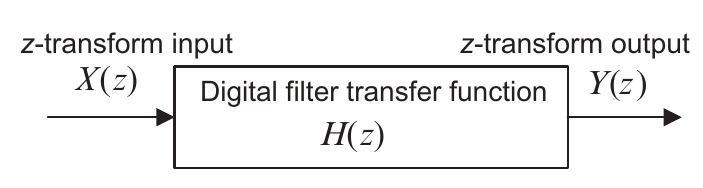
\includegraphics[width=0.3\linewidth]{img/img02}
		\end{center}
		\item can be expanded as
		\begin{center}
			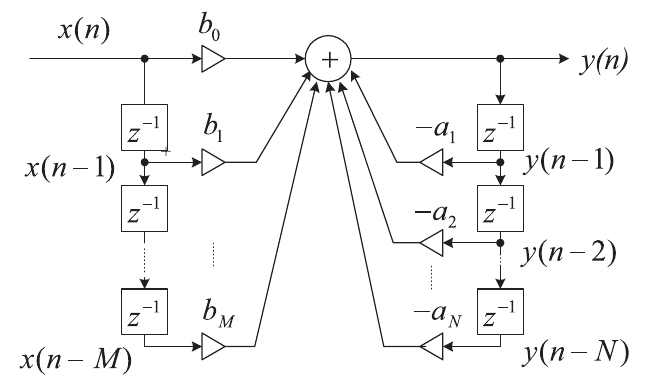
\includegraphics[width=0.7\linewidth]{img/img03}
		\end{center}
		\item if we split:
		\begin{center}
			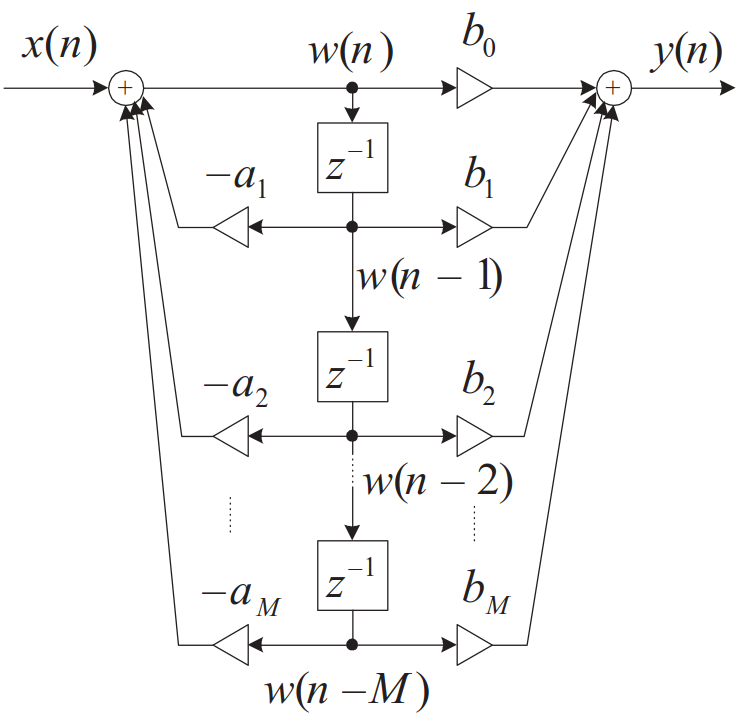
\includegraphics[width=0.7\linewidth]{img/img04}
		\end{center}
	\end{itemize}
\end{frame}

\begin{frame}{Decimation-in-frequency algorithm}
	\begin{itemize}
		\item equation:
		\begin{center}
			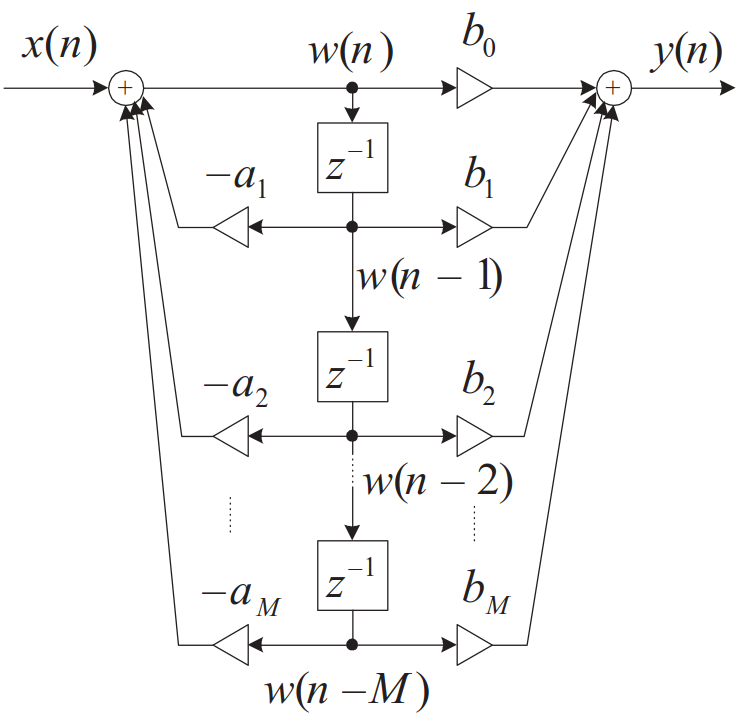
\includegraphics[width=0.7\linewidth]{img/img04}
		\end{center}
		\item can be rewriten as a sum of the following two parts:
		\begin{center}
			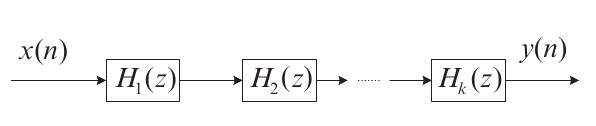
\includegraphics[width=0.7\linewidth]{img/img05}
		\end{center}
	\end{itemize}
\end{frame}

\begin{frame}{Decimation-in-frequency algorithm}
	\begin{itemize}
		\item equation
		\begin{center}
			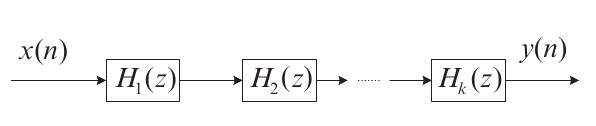
\includegraphics[width=0.6\linewidth]{img/img05}
		\end{center}
		\item modifying the second term:
		\begin{center}
			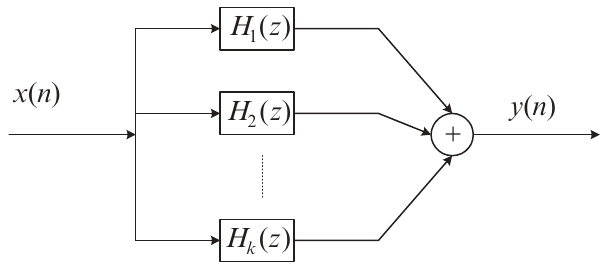
\includegraphics[width=0.7\linewidth]{img/img06}
		\end{center}
	\end{itemize}
\end{frame}

\begin{frame}{Decimation-in-frequency algorithm}
	\begin{itemize}
		\item because
		\begin{center}
			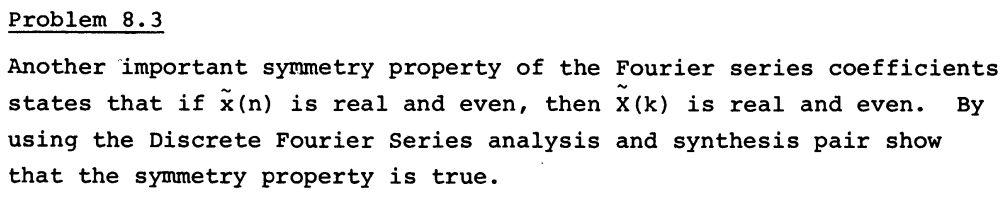
\includegraphics[width=0.5\linewidth]{img/img07}
		\end{center}
		\item then
		\begin{center}
			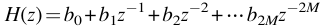
\includegraphics[width=0.7\linewidth]{img/img08}
		\end{center}
	\end{itemize}
\end{frame}

\begin{frame}{Decimation-in-frequency algorithm}
	\begin{itemize}
		\item $k = 2m$ as an even number:
		\begin{center}
			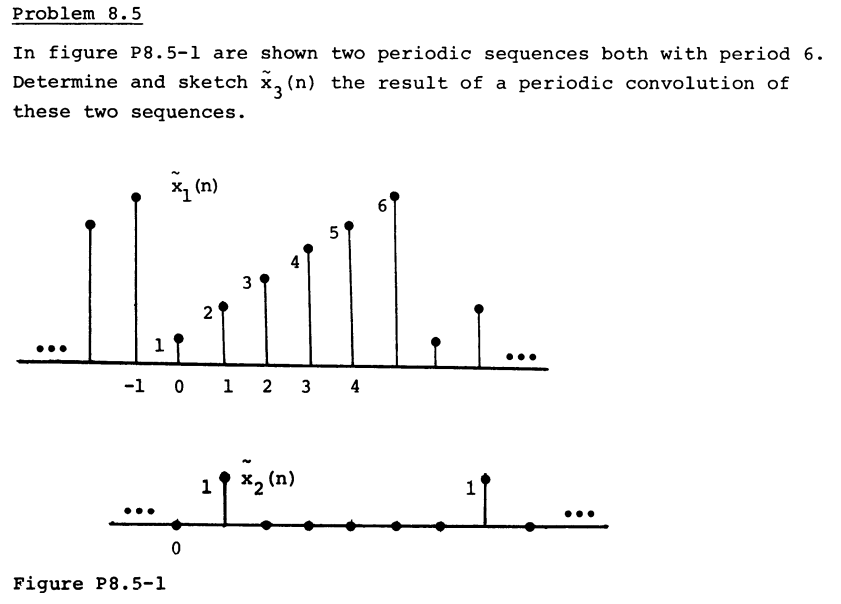
\includegraphics[width=0.7\linewidth]{img/img09}
		\end{center}
		\item $k = 2m+1$ as an odd number:
		\begin{center}
			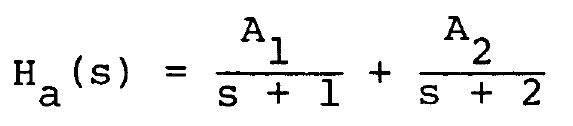
\includegraphics[width=0.7\linewidth]{img/img10}
		\end{center}
	\end{itemize}
\end{frame}

\begin{frame}{Decimation-in-frequency algorithm}
	\begin{itemize}
		\item because
		\begin{center}
			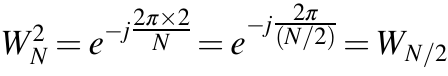
\includegraphics[width=0.5\linewidth]{img/img11}
		\end{center}
		\item then
		\begin{center}
			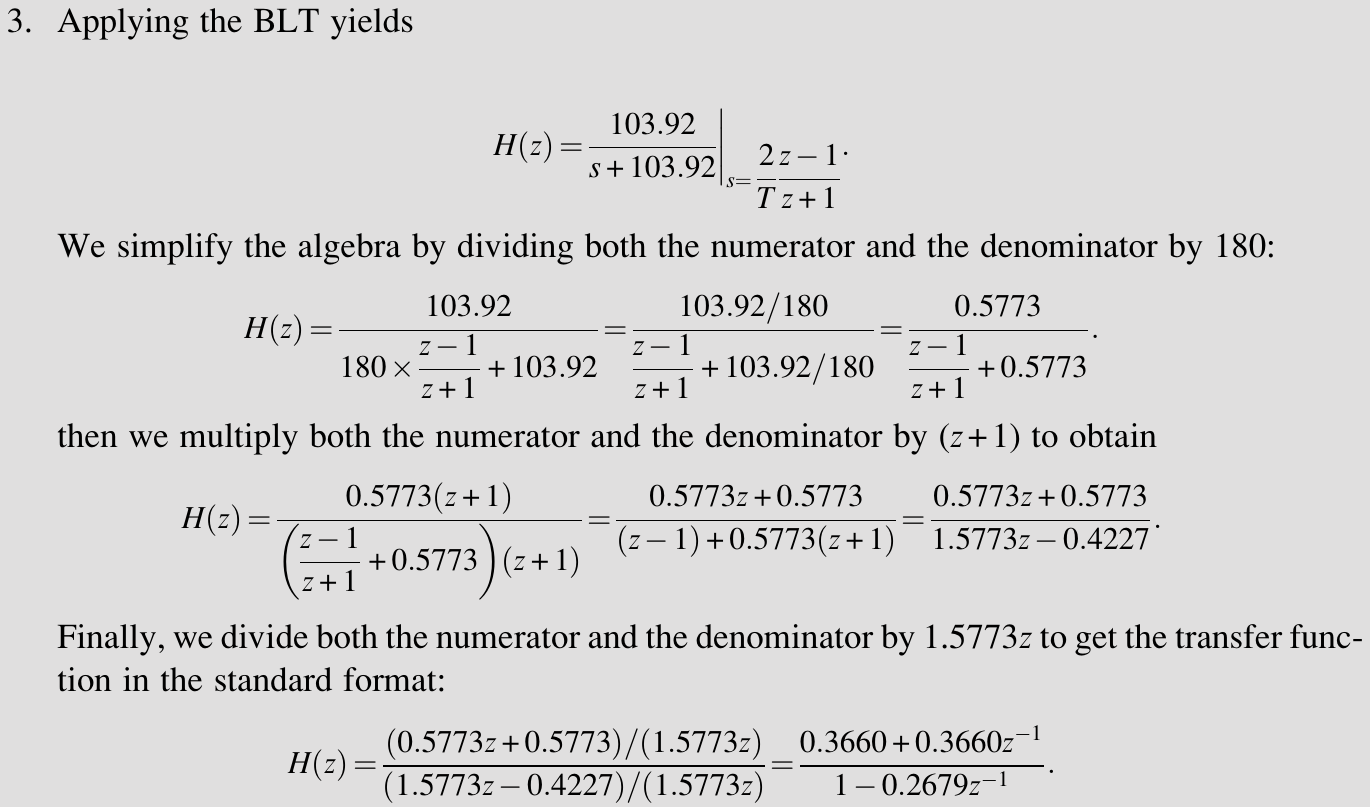
\includegraphics[width=\linewidth]{img/img12}
		\end{center}
	\end{itemize}
\end{frame}

\begin{frame}{Decimation-in-frequency algorithm}
	\begin{itemize}
		\item equation:
		\begin{center}
			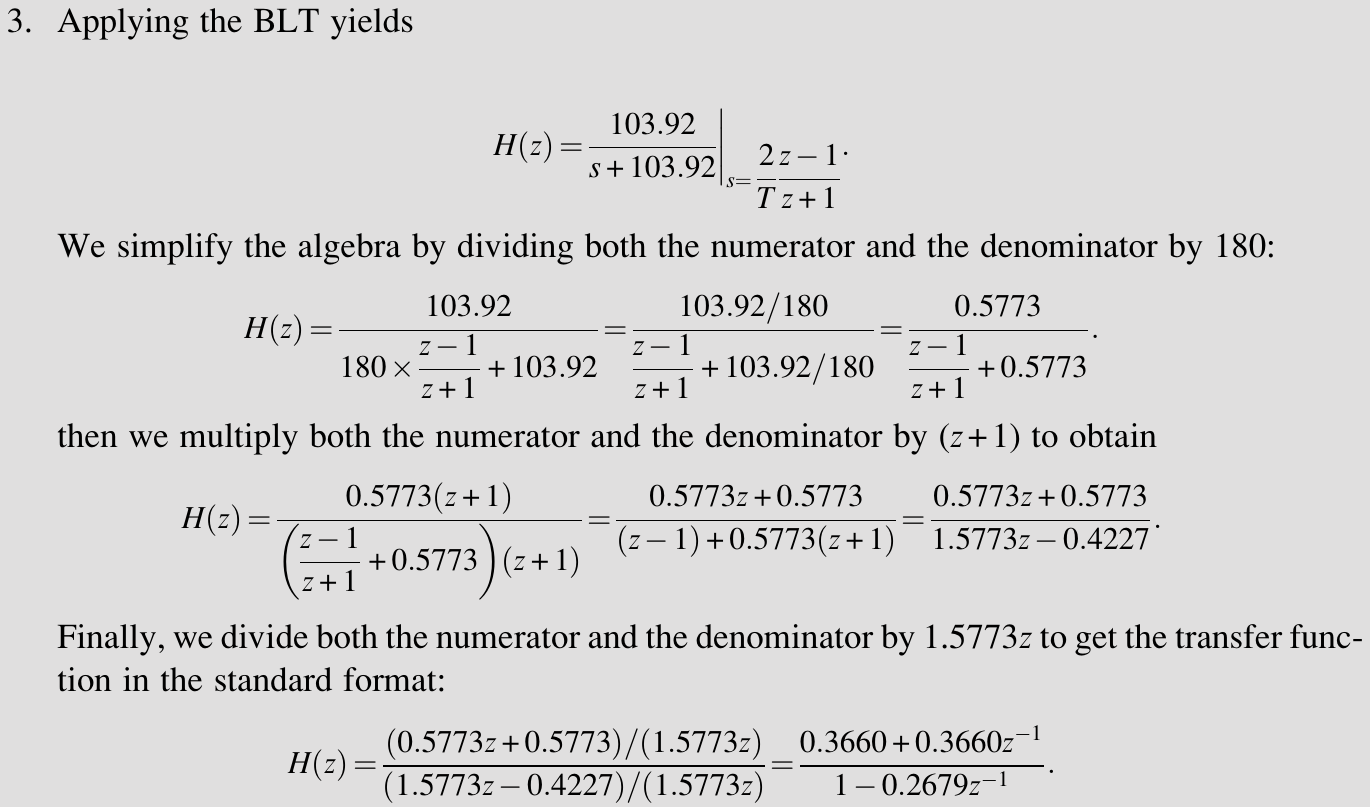
\includegraphics[width=\linewidth]{img/img12}
		\end{center}
		\item where $a(n)$ and $b(n)$ are introduced and expressed as
		\begin{center}
			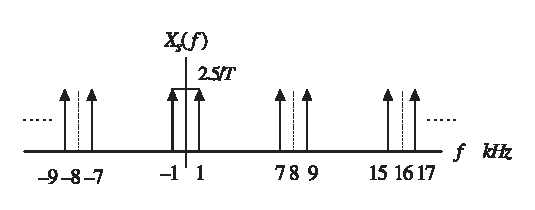
\includegraphics[width=0.7\linewidth]{img/img13}
		\end{center}
	\end{itemize}
\end{frame}

\begin{frame}{Decimation-in-frequency algorithm}
	\begin{itemize}
		\item can be summarized as
		\begin{center}
			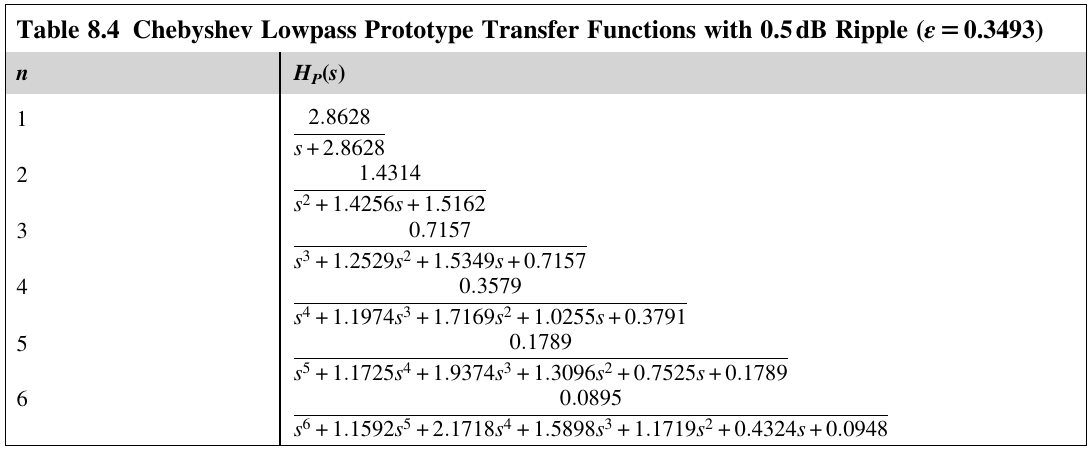
\includegraphics[width=\linewidth]{img/img14}
		\end{center}
		\item comparison
		\begin{center}
			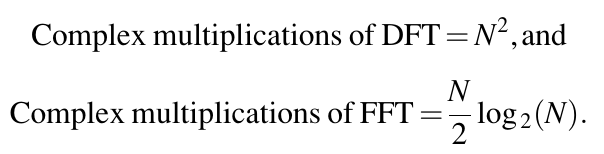
\includegraphics[width=0.7\linewidth]{img/img14a}
		\end{center}
	\end{itemize}
\end{frame}

\begin{frame}{Decimation-in-frequency algorithm}
	\begin{itemize}
		\item The first iteration of the eight-point FFT
		\begin{center}
			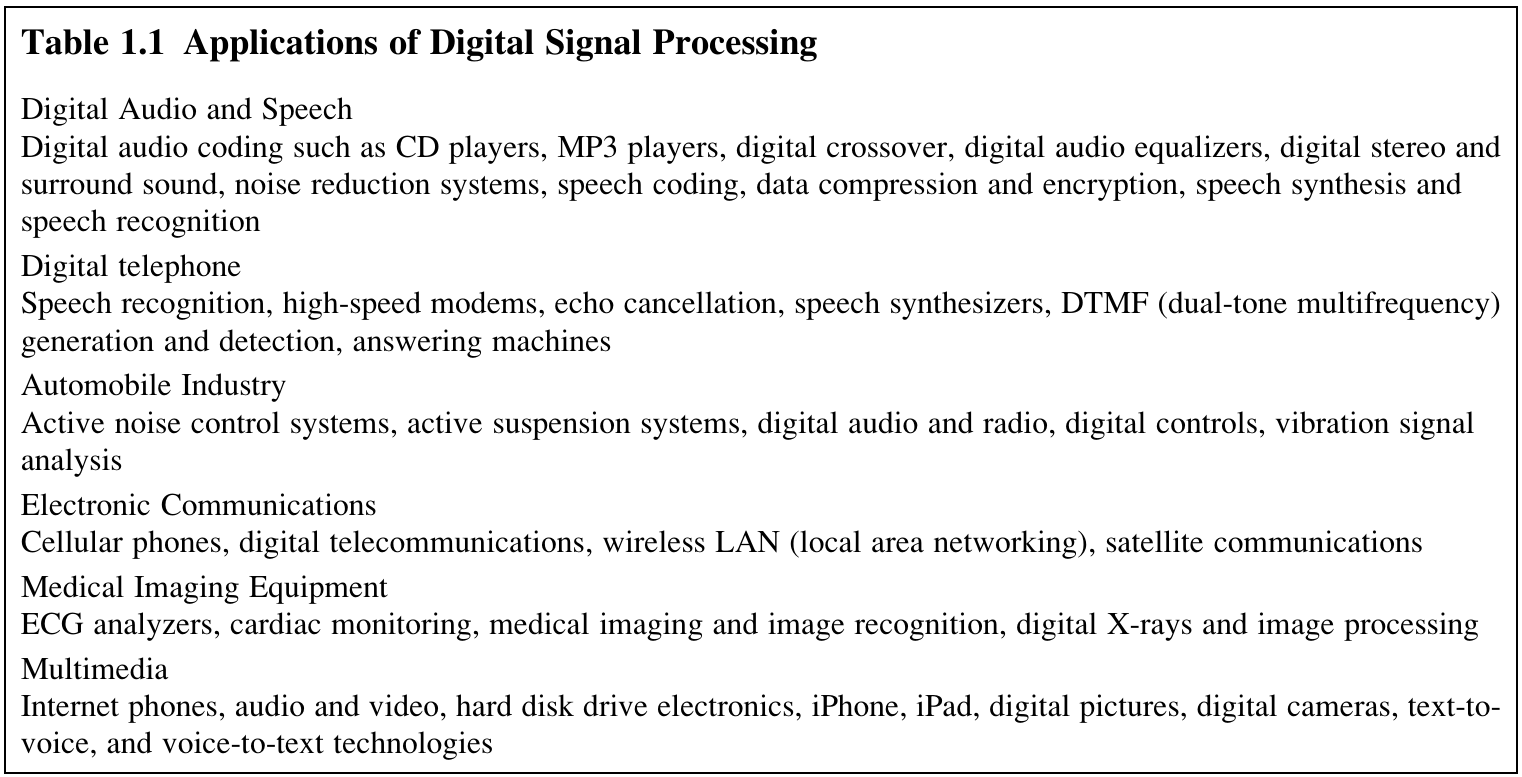
\includegraphics[width=\linewidth]{img/img15}
		\end{center}
	\end{itemize}
\end{frame}

\begin{frame}{Decimation-in-frequency algorithm}
	\begin{itemize}
		\item The second iteration of the eight-point FFT
		\begin{center}
			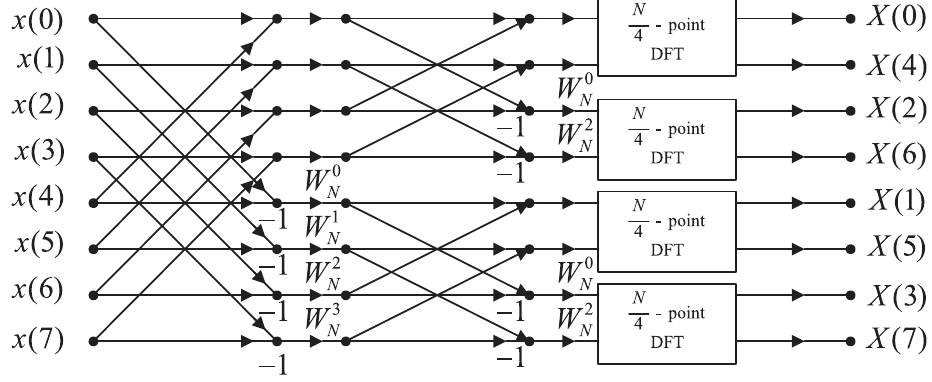
\includegraphics[width=\linewidth]{img/img16}
		\end{center}
	\end{itemize}
\end{frame}

\begin{frame}{Decimation-in-frequency algorithm}
	\begin{itemize}
		\item Block diagram for the eight-point FFT (total 12 multiplications).
		\begin{center}
			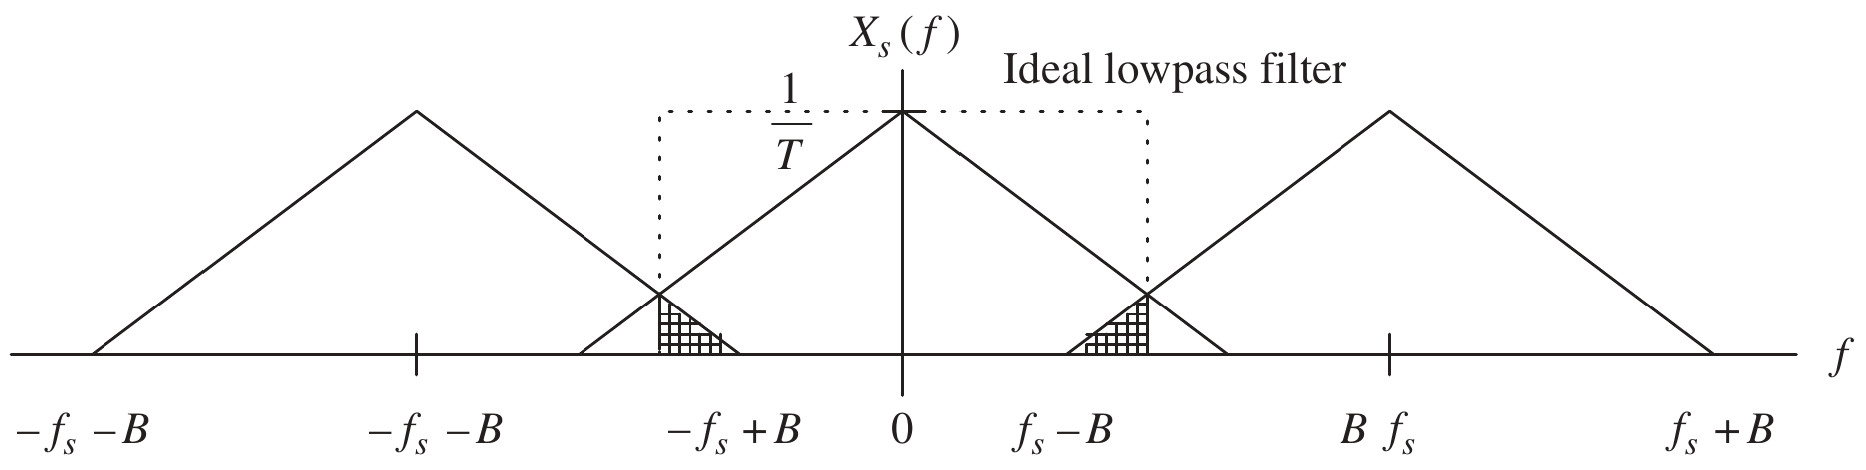
\includegraphics[width=\linewidth]{img/img17}
		\end{center}
	\end{itemize}
\end{frame}

\begin{frame}{Decimation-in-frequency algorithm}
	\begin{center}
		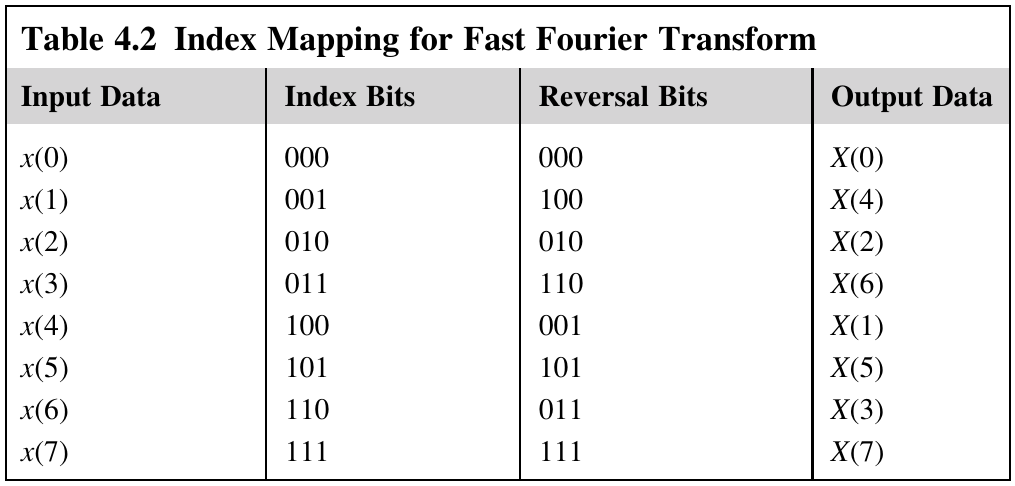
\includegraphics[width=\linewidth]{img/img17a}
	\end{center}
\end{frame}

\begin{frame}{Decimation-in-frequency algorithm}
	\begin{center}
		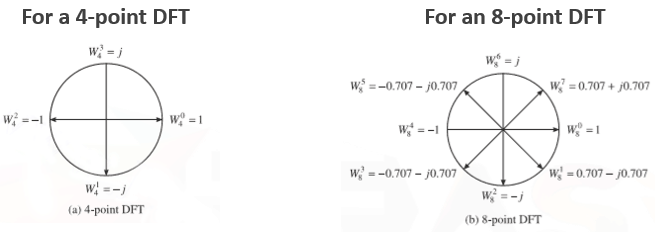
\includegraphics[width=\linewidth]{img/img17b}
	\end{center}
\end{frame}

\begin{frame}{Decimation-in-frequency algorithm}
	\begin{itemize}
		\item Inverse FFT:
		\begin{center}
			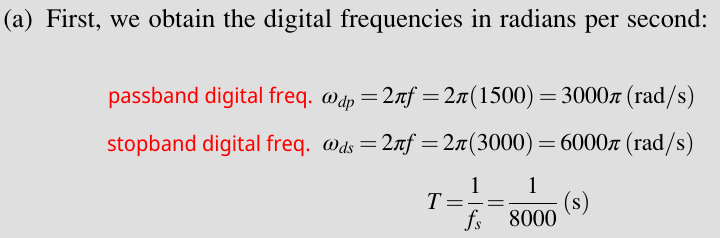
\includegraphics[width=\linewidth]{img/img18}
		\end{center}
	\end{itemize}
\end{frame}

\begin{frame}{Decimation-in-frequency algorithm}
	\begin{itemize}
		\item Inverse FFT:
		\begin{center}
			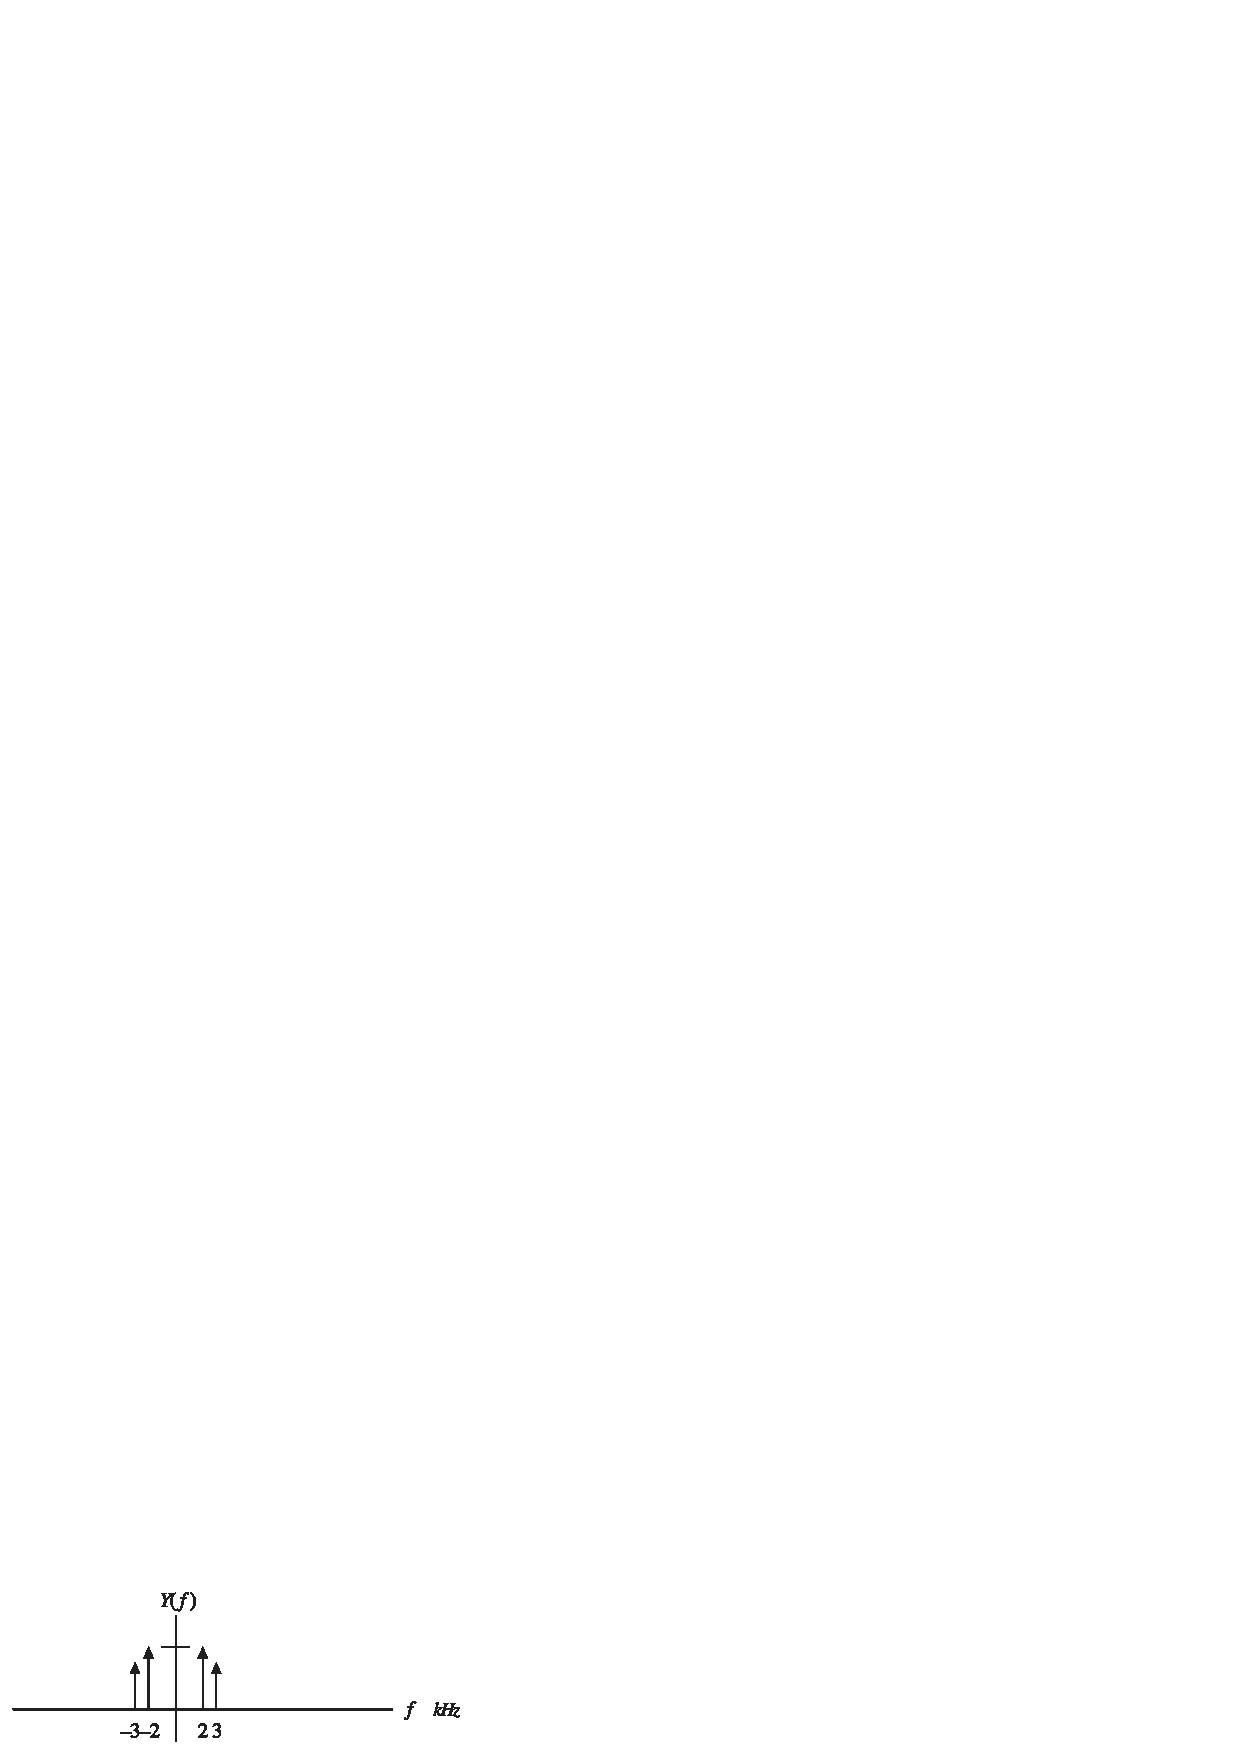
\includegraphics[width=\linewidth]{img/img19}
		\end{center}
	\end{itemize}
\end{frame}

\begin{frame}{Example 1}
	Given a sequence $x(n)$ for $0 \leq n \leq 3$, where $x(0) = 1$, $x(1) = 2$, $x(2) = 3$, and $x(3) = 4$, evaluate its DFT $X(k)$ using the decimation-in-frequency FFT method.
\end{frame}

\section{Decimation-in-time algorithm}

\begin{frame}{Decimation-in-time algorithm}
	\begin{itemize}
		\item we split the input sequence $x(n)$ into the even indexed $x(2m)$ and $x(2m + 1)$, each with $N$ data points
		\begin{center}
			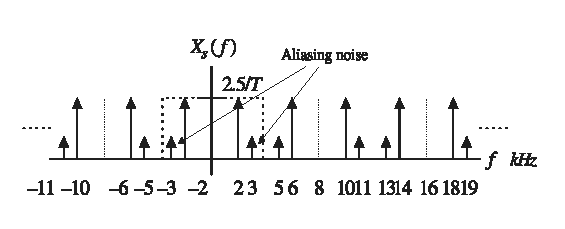
\includegraphics[width=\linewidth]{img/img20}
		\end{center}
		\item because
		\begin{center}
			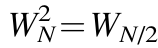
\includegraphics[width=0.2\linewidth]{img/img21}
		\end{center}
		\item then
		\begin{center}
			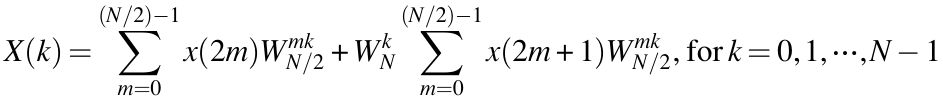
\includegraphics[width=\linewidth]{img/img22}
		\end{center}
	\end{itemize}
\end{frame}

\begin{frame}{Decimation-in-time algorithm}
	\begin{itemize}
		\item equation:
		\begin{center}
			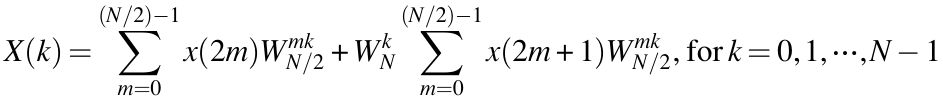
\includegraphics[width=\linewidth]{img/img22}
		\end{center}
		\item define as new function:
		\begin{center}
			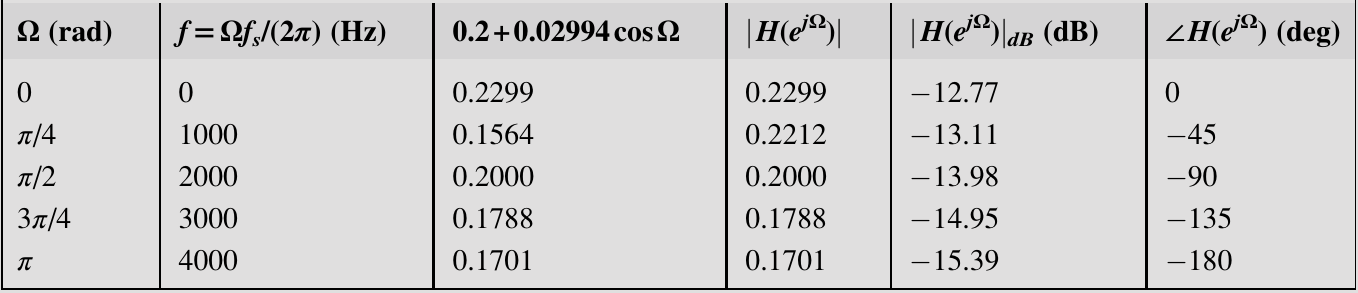
\includegraphics[width=\linewidth]{img/img23}
		\end{center}
	\end{itemize}
\end{frame}

\begin{frame}{Decimation-in-time algorithm}
	\begin{itemize}
		\item note that:
		\begin{center}
			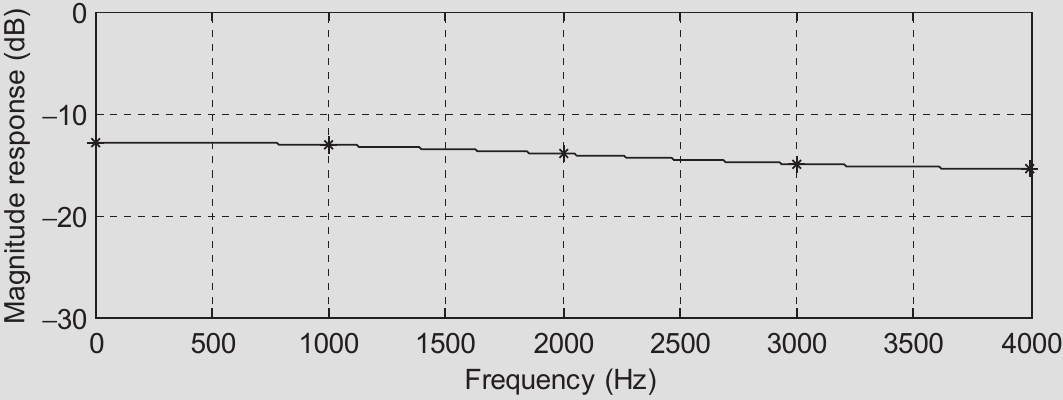
\includegraphics[width=0.6\linewidth]{img/img24}
		\end{center}
		\item then:
		\begin{center}
		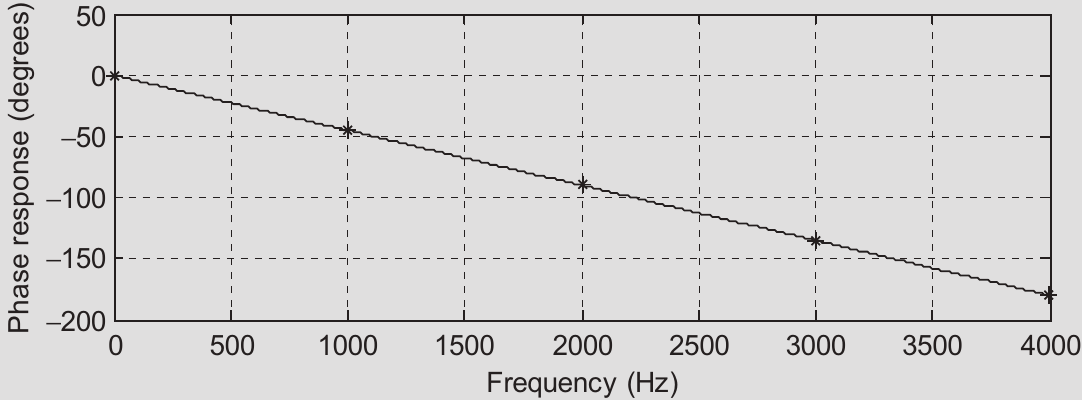
\includegraphics[width=0.8\linewidth]{img/img25}
		\end{center}
	\end{itemize}
\end{frame}

\begin{frame}{Decimation-in-time algorithm}
	\begin{itemize}
		\item note that:
		\begin{center}
			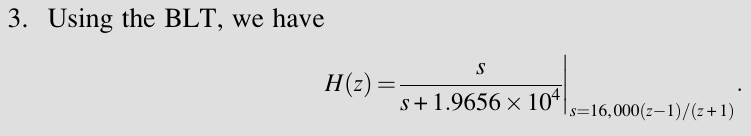
\includegraphics[width=0.3\linewidth]{img/img26}
		\end{center}
		\item then:
		\begin{center}
			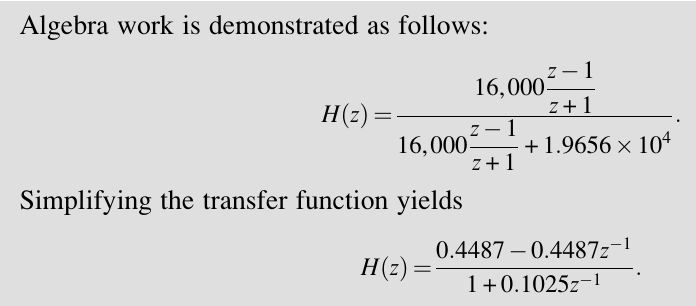
\includegraphics[width=0.8\linewidth]{img/img27}
		\end{center}
	\end{itemize}
\end{frame}

\begin{frame}{Decimation-in-time algorithm}
	\begin{itemize}
		\item the block diagram for the eight-point FFT algorithm (First iteration)
		\begin{center}
			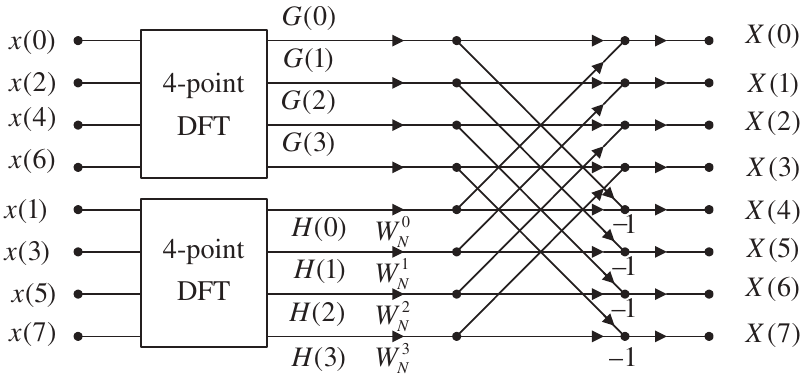
\includegraphics[width=\linewidth]{img/img28}
		\end{center}
	\end{itemize}
\end{frame}

\begin{frame}{Decimation-in-time algorithm}
	\begin{itemize}
		\item the block diagram for the eight-point FFT algorithm (Second iteration)
		\begin{center}
			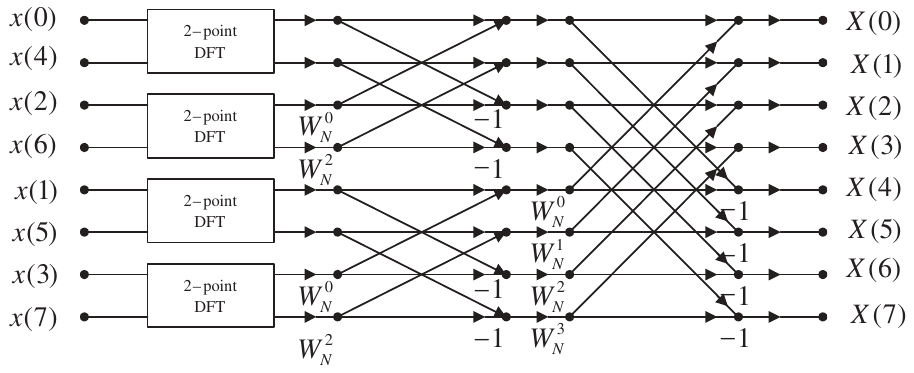
\includegraphics[width=\linewidth]{img/img29}
		\end{center}
	\end{itemize}
\end{frame}

\begin{frame}{Decimation-in-time algorithm}
	\begin{itemize}
		\item Eight-point FFT algorithm using decimation-in-time (12 complex multiplications).
		\begin{center}
			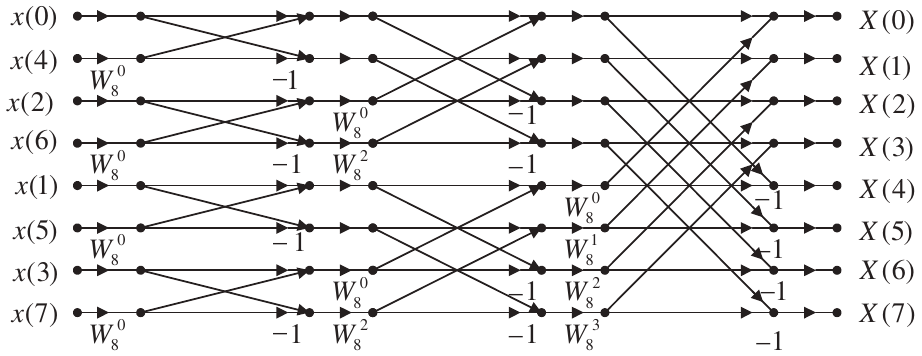
\includegraphics[width=\linewidth]{img/img30}
		\end{center}
	\end{itemize}
\end{frame}

\begin{frame}{Decimation-in-time algorithm}
	\begin{itemize}
		\item The eight-point IFFT using decimation-in-time.
		\begin{center}
			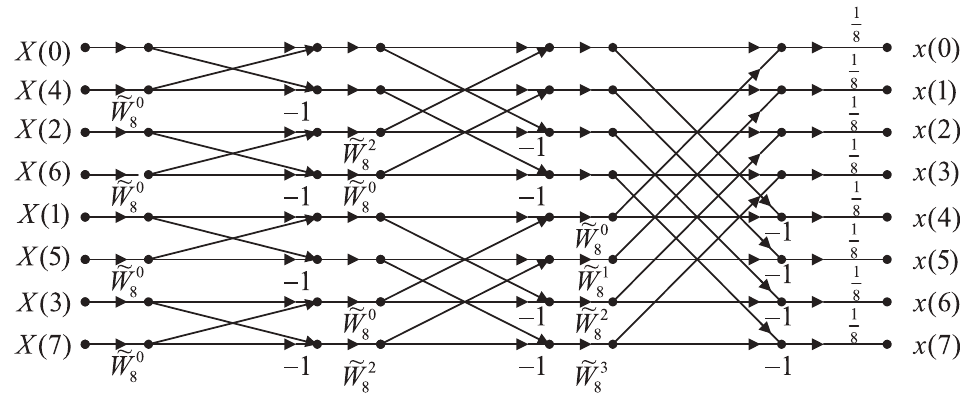
\includegraphics[width=\linewidth]{img/img31}
		\end{center}
	\end{itemize}
\end{frame}

\begin{frame}{Example 2}
	Given a sequence $x(n)$ for $0 \leq n \leq 3$, where $x(0) = 1$, $x(1) = 2$, $x(2) = 3$, and $x(3) = 4$, evaluate its DFT $X(k)$ using the decimation-in-time FFT method.
\end{frame}

\begin{frame}{Fast Fourier Transform}
	\begin{itemize}
		\item frequency resolution, $\Delta f = \frac{f_s}{N}$
		\item frequency bin, $f = \frac{kf_s}{N}$
		\item amplitude spectrum,
		\begin{align*}
			A_k = \frac{1}{N}|X(k)| &= \frac{1}{N}\sqrt{(\text{Real}[X(k)])^2 + (\text{Imag}[X(k)])^2},\\
			&k=0,1,2,\cdots,N-1
		\end{align*}
		for one-sided amplitude spectrum
		\begin{align*}
			\bar{A}_k = \begin{cases}
				\frac{1}{N}|X(0)|,~k=0 \\
				\frac{2}{N}|X(0)|,~k=1,2,\cdots,N/2 \\
			\end{cases}
		\end{align*}
	\end{itemize}
\end{frame}

\begin{frame}{Fast Fourier Transform}
	\begin{itemize}
		\item phase spectrum,
		\begin{align*}
			\varphi_k = \tan^{-1}\left(\frac{\text{Imag}[X(k)]}{\text{Real}[X(k)]}\right),~k=0,1,2,\cdots,N-1
		\end{align*}
		\item power spectrum,
		\begin{align*}
			P_k = \frac{1}{N^2}|X(k)|^2 &= \frac{1}{N^2}\sqrt{(\text{Real}[X(k)])^2 + (\text{Imag}[X(k)])^2},\\
			k&=0,1,2,\cdots,N-1
		\end{align*}
		for one-sided power spectrum
		\begin{align*}
			\bar{P}_k = \begin{cases}
				\frac{1}{N^2}|X(0)|,~k=0 \\
				\frac{2}{N^2}|X(0)|,~k=1,2,\cdots,N/2 \\
			\end{cases}
		\end{align*}
	\end{itemize}
\end{frame}

\end{document}